
79, 78, 82,333

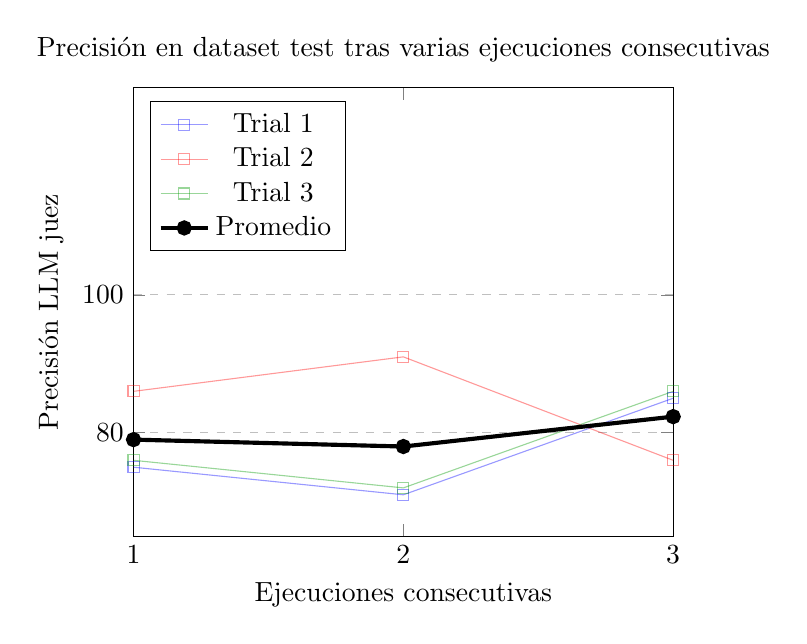
\begin{tikzpicture}
\begin{axis}[
    title={Precisión en dataset test tras varias ejecuciones consecutivas},
    xlabel={Ejecuciones consecutivas},
    ylabel={Precisión LLM juez},
    xmin=1, xmax=3,
    ymin=65, ymax=130,
    xtick={1, 2, 3},
    ytick={0,20,40,60,80,100},
    legend pos=north west,
    ymajorgrids=true,
    grid style=dashed,
]
% Gráfico original de solubilidad
\addplot[
    color=blue,
    mark=square,
    opacity=0.4,
    ]
    coordinates {
    (1, 75)(2, 71)(3, 85)
    };
% Primer punto adicional 
\addplot[
    color=red,
    mark=square,
    opacity=0.4,
    ]
    coordinates {
      (1, 86)(2, 91)(3, 76)
    };
% Segundo punto adicional 
\addplot[
    color=green!60!black,
    mark=square,
    opacity=0.4,
    ]
    coordinates {
      (1, 76)(2, 72)(3, 86)
    };
% Línea promedio
\addplot[
    color=black,
    mark=*,
    line width=1.5pt,
    ]
    coordinates {
      (1, 79)(2, 78)(3, 82.333)
    };
\legend{Trial 1, Trial 2, Trial 3, Promedio}
    
\end{axis}
\end{tikzpicture}

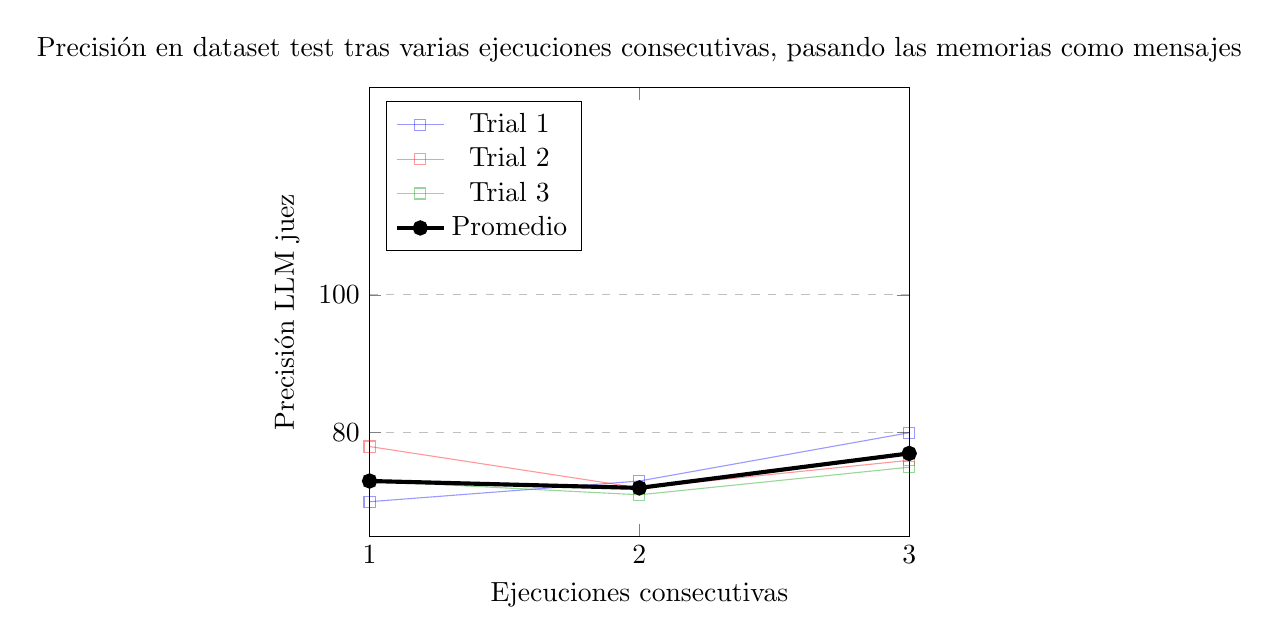
\begin{tikzpicture}
\begin{axis}[
    title={Precisión en dataset test tras varias ejecuciones consecutivas, pasando las memorias como mensajes},
    xlabel={Ejecuciones consecutivas},
    ylabel={Precisión LLM juez},
    xmin=1, xmax=3,
    ymin=65, ymax=130,
    xtick={1, 2, 3},
    ytick={0,20,40,60,80,100},
    legend pos=north west,
    ymajorgrids=true,
    grid style=dashed,
]
% Gráfico original de solubilidad
\addplot[
    color=blue,
    mark=square,
    opacity=0.4,
    ]
    coordinates {
    (1, 70)(2, 73)(3, 80) 
    };
% Primer punto adicional 
\addplot[
    color=red,
    mark=square,
    opacity=0.4,
    ]
    coordinates {
      (1, 78)(2, 72)(3, 76)
    };
% Segundo punto adicional 
\addplot[
    color=green!60!black,
    mark=square,
    opacity=0.4,
    ]
    coordinates {
      (1, 73)(2, 71)(3, 75)
    };
% Línea promedio
\addplot[
    color=black,
    mark=*,
    line width=1.5pt,
    ]
    coordinates {
      (1, 73)(2, 72)(3, 77)
    };
\legend{Trial 1, Trial 2, Trial 3, Promedio}
    
\end{axis}
\end{tikzpicture}

media sin memorias: 76
con memorias train: 81, 83,78 
media con memorias train: 80.66

